\documentclass[a4paper]{oblivoir}
% define the title
\author{Moon Il-chul \\ \href{mailto:icmoon@kaist.ac.kr}{icmoon@kaist.ac.kr} 
   \and Jang Jae-kwan \\ \href{mailto:jgfd123@gmail.com}{jgfd123@gmail.com} }
\setcounter{chapter}{3}
\title{Chapter 3. 나이브 베이즈 분류기}
\usepackage{indentfirst}
\usepackage{graphicx}
\graphicspath{ {Figure/} }
\usepackage{hyperref}
\usepackage{amsmath}
\usepackage{amssymb}
\usepackage{amsfonts}
\usepackage{dsfont}
\usepackage[]{algorithm2e}
\usepackage{chngcntr}
\counterwithin{figure}{chapter}
\setcounter{tocdepth}{2}
\setcounter{secnumdepth}{3}
\hypersetup{pdfborder={0 0 0}}
\renewcommand{\thefigure}{\thechapter-\arabic{figure}}
\renewcommand{\theequation}{\thechapter.\arabic{equation}}
\newlength\myindent
\setlength\myindent{5em}

\begin{document}
% generates the title
\maketitle
%\renewcommand{\contentsname}{목차}
\tableofcontents
%\listoftables
%\listoffigures

% 슬라이드 4
\section{최적 분류법(Optimal Classification)}
\begin{figure}[ht]\centering

\includegraphics[scale=0.5]{Supervised_Learning}\caption{지도학습}\label{Fig:3-1}
\end{figure}
기계학습은 크게 분류(Classification)와 군집화(Clustering) 두 개의 분야로 나눠진다고 했다. 이제 앞으로 먼저 분류(Classification)인 지도학습(Supervised Learning)에 대해서 알아보도록 하겠다. 지도학습에 대해 간단히 다시 짚고 넘어가보자면, 지도학습은 실제 값을 알고 있고 몇가지 예시를 학습에 제공할 수 있는 상황이다. 스팸 필터링이나 자동 등급화, 자동 범주화 같은 경우가 지도학습의 예시이다. 앞서 1장의 1.2 기계학습 종류 부분에 지도학습에 대한 설명이 있으니 기억이 나지 않는다면 참고하길 바란다. 지도학습 중 회귀분석(Regression)도 포함되지만 이 책에서는 다루지 않도록 하겠다. 먼저 최적 분류법(Optimal Classification)에 대한 개념에 대해 알아보도록 하겠다.\\

% 슬라이드 5
\subsection{최적 예측기(Optimal predictor)}
\begin{figure}[ht]\centering
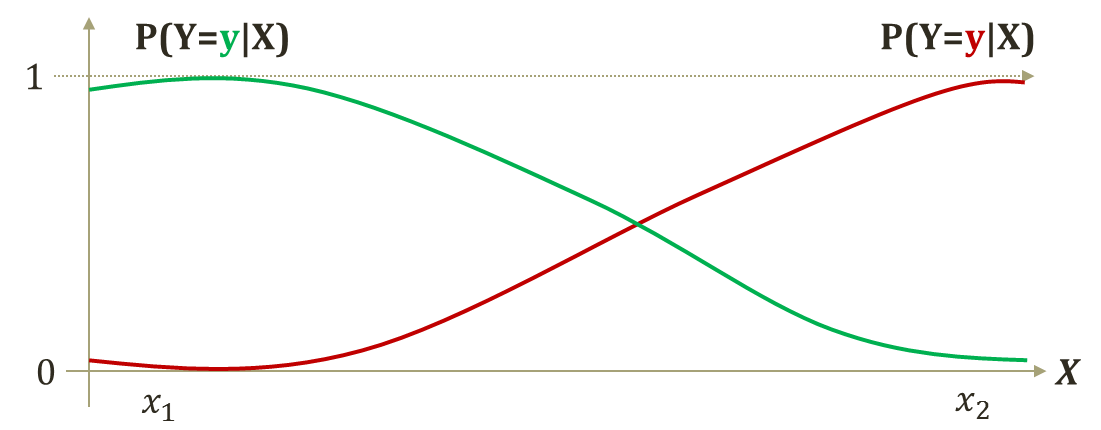
\includegraphics[scale=0.5]{Optimal_predictor}\caption{2개 클래스의 확률밀도함수}\label{Fig:3-2}
\end{figure}
그림 2는 X라는 정보가 조건으로 주어졌을 때, Y 값이 어떤 값인지 알아보는 그림이다. 만약 X가 $x_1$에서 관측이 되었다고 한다면($X=x_1$), 이 경우 Y가 초록색 y가 될 확률은 매우 높다. 반면 Y가 빨간색 y가 될 확률은 매우 낮다. 이를 통해 우리는 Y가 초록색 y라고 하는 것이 더 낫다고 얘기할 수 있다. 상황이 바뀌어서 만약 X가 $x_2$에서 관측이 되었다고 한다면($X=x_2$), Y가 빨간색 y일 확률이 높고 초록색 y일 확률이 낮다. 따라서 이 경우에는 Y가 빨간색 y라고 하는 것이 좋다고 말할 수 있다. 즉, X라는 조건이 어떻게 주어졌는 지에 따라 Target Class인 Y의 확률 값을 계산해주어야 한다. 이를 위해서 두 개의 클래스에 대한 확률밀도함수(PDF)를 정의를 할 수 있다면 좋을 것이다. 그래서 우리는 Bayes Classifier(베이즈 분류기)라는 것을 정의할 것이다. 베이즈 분류기의 Optimal predictor는 다음과 같다.
\begin{equation}
f^*={argmax}_{f}P(f(X) \neq Y)
\label{eq:3-1}
\end{equation}
\indent이 식의 의미를 알아보도록 하겠다. 먼저 f(X)는 y를 예측하게 된다. 하지만 이 예측한 y는 error가 있을 수 있으므로 실제값이 다른 $\hat{y}$ 값이 된다. 즉, 우변의 의미는 $\hat{y}\neq Y$의 확률을 최소화(argmin) 하는 f를 찾는 것이고 그 값을 $f^*$라고 하겠다는 말이다. 이 수식은 error를 최소화 하기 위해 함수 근사화를 하는 것이다.\\
\indent 만약 여기에서 그림 2와 같이 두 개의 클래스만 있다고 가정한다면, X 값이 주어졌을 때 $P(f(X)\neq Y)$를 최소화 하는 값은 $P(Y=y|X=x)$를 최대화 하는 값과 같으므로 $f^*$는 다음과 같이 나타낼 수 있다.
\begin{align}
&f^*(x)={argmax}_{Y=y}P(Y=y|X=x)\label{eq:3-2}\\
&\sum_{y \in Y} P(Y=y|X=x)=?\label{eq:3-3}
\end{align}
\indent 즉 X가 $x_1$의 값이 나올 때는 Y가 초록색 y로 예측되고, X가 $x_2$의 값일 때는 Y가 빨간색 y로 예측될 수 있도록 확률밀도함수를 조정하는 역할이 $f^*(x)$이다. \\\\

% 슬라이드 6
\indent 이는 결국 확률에 관한 이야기가 된다. 앞서 1장에서 압정 던지는 문제로 알아본 확률 계산을 하는 방법은 2가지가 있었다. MLE와 MAP 방법이 있다. 먼저 MLE는 관측된 값만 활용하여 $\hat{\theta}$를 구했었다.
\begin{align}
&\hat{\theta}={argmax}_{\theta}P(D| \theta)\label{eq:3-4}\\
&P(D| \theta)=\theta^{a_H}(1-\theta)^{a_T}\label{eq:3-5}\\
&\hat{\theta}=\frac{a_H}{a_H+a_T}\label{eq:3-6}
\end{align}
\indent MAP의 경우에는 사전지식인 $\alpha$와 $\beta$를 활용하여 $\hat{\theta}$를 구했다. 우리는 MLE와 MAP를 구한 과정을 참고하여 분류기(Classifier)를 구하는데 활용할 것이다.
\begin{align}
&\hat{\theta}={argmax}_{\theta}P(\theta|D)\label{eq:3-7}\\
&P(\theta| D) \propto \theta^{a_H+\alpha-1}(1-\theta)^{a_T+\beta-1}\label{eq:3-8}\\
&\hat{\theta}=\frac{a_H+\alpha-1}{a_H+\alpha+a_T+\beta=2}\label{eq:3-9}
\end{align}
\\
\indent 예를 들어, Y값이 \{H,T\}로 두 개의 클래스를 갖는다고 가정해보자. 그리고 $\theta$는 head가 나올 확률이라고 하고, X=D로써 이전의 시도로 구한 데이터셋이라고 해보자. 이 경우 다음과 같은 식을 얻을 수 있다.
\begin{align}
&\hat{\theta}={argmax}_{\theta} P(\theta| D) \label{eq:3-10}\\
&\rightarrow f^*(x)={argmax}_{Y=y}P(Y=y|X) \label{eq:3-11}
\end{align}
여기서 수식 \eqref{eq:3-10}에서는 User가 $\hat{\theta}>0.5$를 가정하면, Y=H라는 결과를 얻게 되지만, 수식 \eqref{eq:3-11}에서는 분류기(Classifier)가 Y=H인지 아닌지를 말을 해준다는 차이가 있다.\\

% 슬라이드 7
\subsection{베이즈 위험(Bayes risk)}
\begin{figure}[ht]\centering
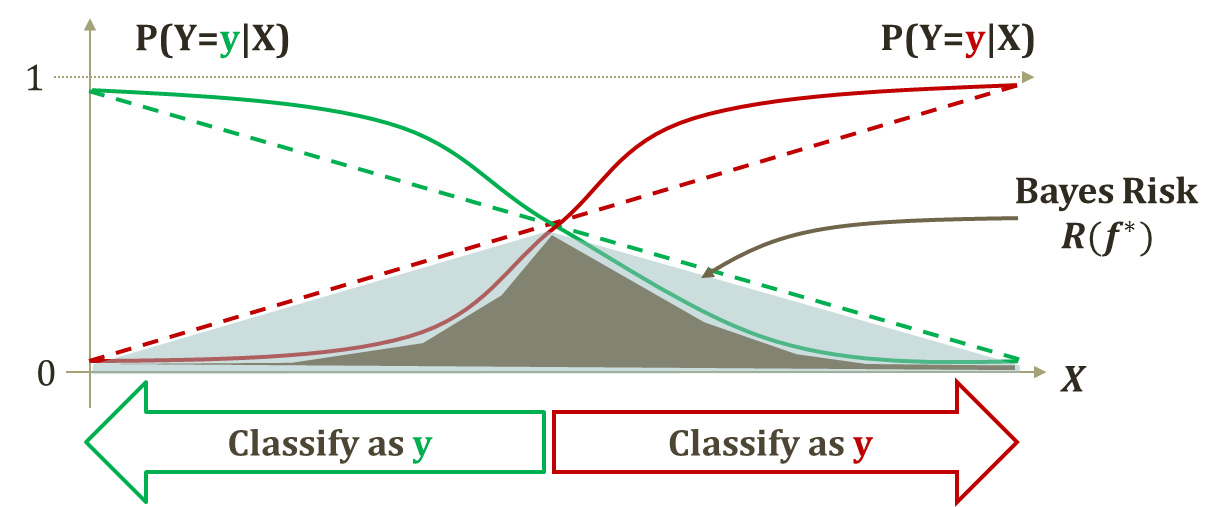
\includegraphics[scale=0.5]{Bayes_Risk}\caption{Bayes Risk}\label{Fig:3-3}
\end{figure}
\indent 이제 MLE와 MAP를 활용하여 좀 더 나은 분류기(Classifier)를 만들 수 있을 지에 대해 다뤄보겠다. 위의 그림은 실선 1쌍과 점선 1쌍으로 이루어진 총 4개의 PDF 함수를 나타낸 것이다. 각 쌍에서 빨간색 선과 초록색 선은 동시에 일어나지 않는다. 그래서 X가  가로축의 어느 한 값 $x_1$을 가질 때, Y가 초록색 y가 될 확률($P_1$)과 빨간색 y가 될 확률($P_2$)을 더한 값은 1이다. 그리고 X의 값에 따라 Y 값을 초록색 y로 분류할지 빨간색 y로 분류할지 결정이 되어진다. 만약 X의 값이 두 실선(점선)의 교점($x_m$)에 해당한다면 $P_1=P_2$로 두 확률 값은 같게 된다. 따라서 Y 값을 분류를 할 수 없게 된다. 여기서 교점 $x_m$을 Decision Boundary라고 하고 뒤에 좀 더 자세히 다루도록 하겠다.\\
\indent 한편 점선의 경우에 X 값이 $x_m$(Decision Boundary) 근처의 값을 가진다면 두 확률의 값이 차이가 크지 않게 되어 Y 값이 초록색일지 빨간색인지 명확하게 높은 확률 차이로 구분을 할 수 없게 된다. 반대로 실선의 경우에는 점선보다는 확률의 차이가 크게 되어 좀 더 높은 확률 차이로 구분을 할 수 있다. 이와 같이 두 확률의 차이가 크지 않다면 Y 값을 분류를 하기가 애매하다. 따라서 점선과 같이 PDF를 설정하는 것보다 실선과 같이 PDF를 설정하여 Decision Boundary 부근에서 확률이 급격히 변하는 것이 분류하는 데 더 용이하다.\\
\indent 그림 3에서 X의 값이 Decision Boundary 왼쪽에 있을 경우 초록색 y로 판별을 하게 된다. 하지만 빨간색 y가 될 확률도 분명히 존재한다. 즉, 빨간선 아래의 부분만큼이 Error가 되는 것이다. 점선의 경우에는 연한 회색 영역+회색 영역, 실선의 경우에는 회색 영역이 Error가 된다. 다시 말해서, 연한 회색 영역 만큼 실선이 더 작은 Error를 가지므로 더 좋은 경우라고 되는 것이다. 그리고 각 경우의 Error 영역을 Bayes Risk($R(f^*)>0$)라고 한다. 대부분 분류기(Classifier)는 실수로 Bayes risk를 갖게 되지만 최적 분류기(Optimal classifier)는 이를 최대한 줄이는 것이 목적이다. 그 이유는 joint probability에 대한 충분한 정보가 없기 때문이다.
\begin{align}
\begin{split}
P(Y=y&|X=x)=\frac{P(X=x|Y=y)p(Y=y)}{P(X=x)}\\
\end{split}\\
\begin{split}
&f^*(x)={argmax}_{Y=y}P(Y=y|X=x)\\
&\ \ \ \ \ \ ={argmax}_{Y=y} P(X=x|Y=y)P(Y=y)
\end{split}
\label{eq:3-13}
\end{align}
\\

% 슬라이드 8
\subsection{결정 경계(Decision boundary)}
\begin{figure}[ht]\centering
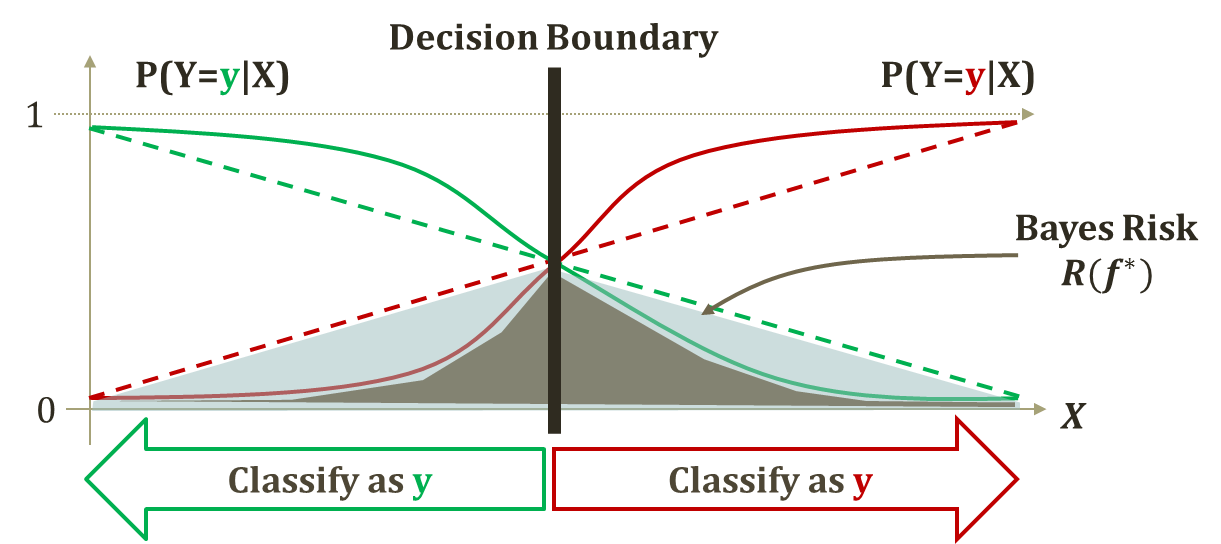
\includegraphics[scale=0.5]{Decision_Boundary1}\caption{결정 경계}\label{Fig:3-4}
\end{figure}
\indent 위의 그림 4 에서 가운데 선부분이 결정 경계가 된다. 그리고 수식 \eqref{eq:3-13}에서 $P(Y=y|X=x)$가 $P(X=x|Y=y)P(Y=y)$ 형태로 바뀌는데 이 두 식은 같은 값은 아니다. 아래 그림 5와 같이 바뀐 수식은 다른 형태의 모양을 가질 수 있다. 이 이유는 두 식이 비례관계인 것이지 정확히 일치하진 않기 때문이다. 또한 주어진 Y의 값이 무엇이냐에 따라서 수식의 값이 달라지기도 한다.
\begin{figure}[ht]\centering
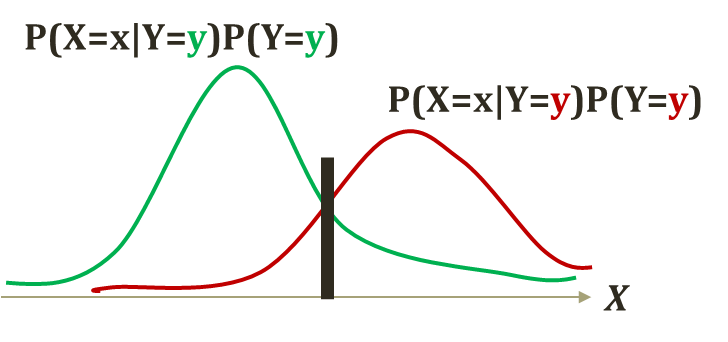
\includegraphics[scale=0.6]{Decision_Boundary2}\caption{조건부 확률의 결정 경계}\label{Fig:3-5}
\end{figure}\\
\indent 예로 정규분포를 들 수 있다. 정규분포의 확률 식은 다음과 같다. 여기서 $\mu$와 $\sigma$는 주어지는 값이다. 그리고 이 값에 따라 정규분포의 확률밀도함수의 형태가 달라진다. 즉 Y의 값($\mu,\sigma$)이 어떻게 주어졌는지에 따라 형태가 달라질 수 있다.
$$P(X=x;\mu ,\sigma)=\frac{1}{\sigma\sqrt{2\pi}}e^{-\frac{(x-\mu)^2}{2\sigma^2}}$$

% 슬라이드 9
\begin{figure}[ht]\centering
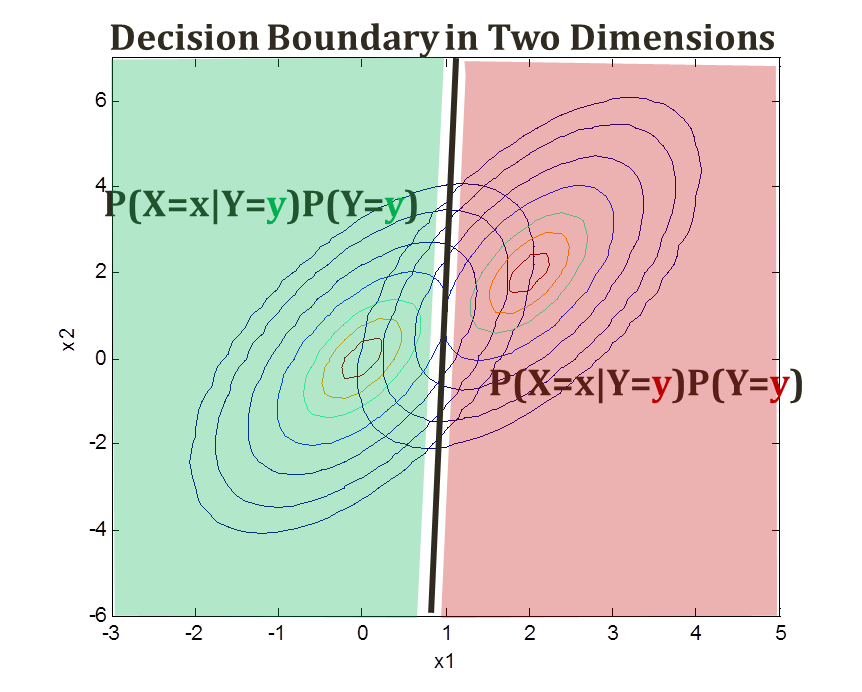
\includegraphics[scale=0.5]{Decision_Boundary3}\caption{2차원에서의 결정 경계}\label{Fig:3-6}
\end{figure}
\indent 결정 경계는 2차원에서도 구할 수 있다. 그림 6과 같이 $x_1,x_2$가 있을 때, 결정 경계는 가운데 검은 선으로 둘 수 있다. 또한 앞에서 예시로 들었던 정규분포에서 2개의 변수를 가지는 다변수 정규분포에 대한 조건부 확률도 구해볼 수 있다. 이 때 결정 경계는 선형으로 나타나게 된다. 그리고 수식으로 나타내면 다음과 같다.
\begin{equation}
\begin{split}
&P(X=x;\mu ,\sigma)=\frac{1}{\sigma\sqrt{2\pi}}e^{-\frac{(x-\mu)^2}{2\sigma^2}}\\
&\ \ \ \ \ \ \ \ \Downarrow\\
&P(X=(x_1,x_2)|Y=y)=\frac{1}{\sqrt{2\pi}| \sum_y |}exp(-\frac{(x-\mu_y)\sum_{y}^{-1}(x-\mu_y)}{2}
\end{split}
\end{equation}
\\\\
% 슬라이드 10
\indent 앞서 Risk를 줄이는 분류기(Classifier)를 만드는 방법에 대해서 배워보았다. 이렇게 분류기(Classifier)를 만들 때 선형으로 만들 수도 있고 곡선형으로 만들 수도 있다. 선형보다는 곡선형이 좀 더 좋다는 내용은 앞에서 언급을 하였다. 이렇게 곡선형으로 만드는 방법에는 뒤에서 배우도록 하겠다. 그 전에 앞서 간단한 분류기(Classifier)를 만드는 방법에 대해 알아보겠다.
\begin{equation}
\begin{split}
f^*(x)&={argmax}_{Y=y}P(Y=y|X=x)\\
&={argmax}_{Y=y} P(X=x|Y=y)P(Y=y)
\end{split}
\end{equation}
\indent 최적 분류기(Optimal Classifier)는 데이터로 주어진 y와 우리가 판별해서 나온 Y가 같은 값이 나올 확률이 최대가 될 수 있도록 만드는 값이다. 위의 수식에서 $P(Y=y|X=x)$ 부분은 사전(Prior) 정보가 들어가지 않았으므로 Bayes theorem을 이용하여 사전 정보가 들어가도록 하여  $P(X=x|Y=y)P(Y=y)$와 같이 바꿀 수 있다. 그 이유는 argmax 함수 안에 있고 두 수식이 비례관계에 있기 때문이다. 여기서 $P(X=x|Y=y)$ 부분은 조건부밀도(Conditional Density) 클래스이고 $P(Y=y)$ 부분은 사전 클래스이다. 이렇게 식을 바꾸고 나면, 우리는 Prior와 Likelihood를 알아야 한다. 
\begin{align}
&Prior=Class\ Prior=P(Y=y)\\
&Likelihood=Class\ Conditional\ Density=P(X=x|Y=y)P(Y=y)
\end{align}
\indent 이 값들은 데이터셋에서 얻은 관측으로 알 수 있다. 위의 값은 X와 Y의 값의 종류가 적을 때는 쉽게 구할 수 있다. 하지만 보통 데이터셋은 X,Y의 값의 종류가 매우 많을 수 있다. 예를 들어, X 값 하나가 사람 한명에 해당한다고 생각하면 X의 키, X의 몸무게, X의 나이 등 여러 요소들이 존재 할 수 있다. 이 경우 데이터셋이 X와 Y값의 모든 결합 가능한 경우들을 다 가지고 있지 않을 수 있다. 이러한 문제점을 해결을 하는 방법이 나이브 베이즈 분류기(Naive Bayes Classifier)가 되겠다.\\\\

% 슬라이드 11
\section{나이브 베이즈 분류기(Naive Bayes Classifier)}
지금부터는 나이브 베이즈 분류기(Naive Bayes Classifier)에 대해서 알아보겠다. 이전 절에서는 최적 분류법(Optimal Classification)의 개념에 대해서 배우면서 Bayes Theorem을 활용하여 $P(Y|X)$ 부분을 $P(X|Y)P(Y)$로 바꿔보았다. 그리고 X값이 여러 개일 때 문제점이 있다는 것 확인했다. 이번 절에서는 나이브 베이즈 분류기(Naive Bayes Classifier)를 활용하여 여러 X 값이 있을 때의 해결 방법에 대해서 고민해 보도록 하겠다.\\

% 슬라이드 12
\subsection{분류기(Classifier)}
\begin{figure}[ht]\centering
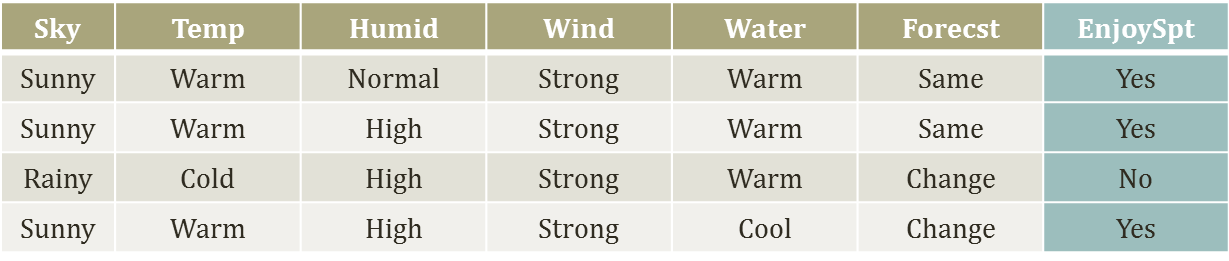
\includegraphics[scale=0.5]{Dataset}\caption{데이터셋}\label{Fig:3-7}
\end{figure}
\indent 위의 데이터셋에서는 X에는 Sky, Temp, Humid, Wind, Water, Forecast로 여러 요소들이 있다. 이때 Y(Enjoyspt)를 어떻게 판별할지 정하는 Classification 문제이다. 최적 분류기(Optimal Classifier)는 다음과 같다고 하였다.
$$f^*(x)={argmax}_{Y=y} P(X=x|Y=y)P(Y=y)$$
여기서 각 성분에 대한 예시를 나타내면 다음과 같다.
\begin{itemize}\setlength\itemsep{-\parsep}
	\item $P(X=x|Y=y)=$
	\begin{description}\setlength\itemsep{-\parsep}
		\item $P$($x_1$=sunny,$x_2$=warm,$x_3$=normal,$x_4$=strong,$x_5$=warm,$x_6$=same$|y$=Yes)
	\end{description}
\end{itemize}
\begin{itemize}\setlength\itemsep{-\parsep}
	\item $P(Y=y)=P(y=$Yes)
\end{itemize}
\indent 이 때 필요한 매개변수의 수는 얼마나 될까? 그리고 얼마나 많은 관측값이 필요할까? \\
\indent 데이터셋에서 X는 d개의 요소를 가지고 있고 각 요소는 2가지 종류의 값을 가진다고 가정을 하고, Y의 값은 k가지 값을 가진다고 가정을 해보자. 그렇다면 $P(Y=y)$는 총 k-1개의 관측값이 필요하다. 그 이유는 k-1개의 종류의 값을 가지면, 전체 확률 1에서 k-1개 종류의 확률을 빼면 가지고 있지 않은 마지막 종류의 확률값을 자동으로 구할 수 있기 때문이다. $P(X=x)$의 경우에는 총 $2^d$ 종류의 값을 가지게 되고 총 $(2^d-1)$개의 관측값이 필요하다. 따라서 $P(X=x|Y=y)$는 총 $(2^d-1)k$개의 관측값이 필요하다. 그림 7의 데이터셋을 통해 확인을 해보면 $P(Y=y)$는 총 1개의 관측값만이 필요하고, $P(X=x|Y=y)$는 총 $(2^6-1)*2=126$개의 관측값이 필요하다.
$$N>>(2^d-1)k>>|D|$$
\indent 여기서 d값이 커지면 필요한 관측값의 수는 급속도로 많아지게 되는 문제점이 생긴다. 그리고 우리는 완벽한 세상에서 살고 있는게 아니기 때문에 노이즈가 존재한다. 따라서 이를 줄이기 위해 확률변수 분포로 모델화하는 것이 필요하고 같은 케이스에 대해서도 여러번 반복하는 것이 필요하다. 실제 세상에서는 X의 요소가 더 많아질 수 있으므로 X의 요소들이 joint 되는 부분을 해결할 필요가 있다.

% 슬라이드 13
\indent 따라서 $f^*(x)={argmax}_{Y=y} P(X=x|Y=y)P(Y=y)$ 와 같은 모델을 배우기 위해서는 아주 많은 데이터 셋이 필요한데, 이를 얻는것은 거의 불가능하다. 이 모델은 비현실성적인 가정을 완화 시켰지만 이제는 모델을 배울 수가 없게 되었다. 따라서 다른 가정이 추가되어야 한다. 이 가정은 완화된 가정과 같이 그렇게 중요하지 않은 가정이어야 한다.\\
\indent 그렇다면 데이터셋의 수요 중 어느 부분이 주요한 요인일까? 바로 $P(X=x|Y=y)$ 부분이다. 
$$P(X=x|Y=y)\ for\ all\ x,y \Rightarrow (2^d-1)k $$
여기서 x는 벡터값으로 벡터의 길이는 d에 해당한다. 그렇지만 d를 줄이는 것은 피하고 싶을 것이다. 왜냐하면 데이터셋을 힘들게 구했는데 얻은 정보를 줄이는 것은 그다지 좋은 선택이 아닐 것이다. 그렇다면 d를 줄이는 방법이 아닌 다른 어떤 방법이 있을까?\\

% 슬라이드 14
\subsection{조건부 독립(Conditional independence)}
그래서 생각을 해본게 조건부 독립(Conditional independence)이란 가정을 도입을 하자는 것이다. 조건부 독립을 적용하면 다음과 같은 결과를 얻을 수 있다.
\begin{equation}
P(X =< x_1,...,x_i>|Y=y)\rightarrow\prod_i P(X_i = x_i|Y =y)
\end{equation}
\indent 위의 수식은 y가 주어졌을 때 $x_1,...,x_i$가 모두 조건부 독립일 때 가능한 결과이다. 쉽게 생각해서 X와 Y가 독립일때 $P(X,Y)=P(X)P(Y)$가 되는 것을 생각하면 된다. 이렇게 했을 때 좋은 점은 $2^d-1$만큼 필요했던 매개변수의 수가 $d$개만 필요하도록 바꿀 수 있다는 것이다. $y$가 주어졌을 때, $x_1$이 $x_2$에 조건부 독립인 경우의 수학적인 정의는 다음과 같다.
\begin{equation}
(\forall x_1,x_2,y)\ \ P(x_1|x_2,y) = P(x_1|y)
\end{equation}
즉, 좌변에서 $x_2$의 조건이 빠져도 우변과 같은 확률이 나오게 된다. 결과적으로 위의 주장은 다음과 같다.
\begin{equation}
P(x_1,x_2|y) = P(x_1|y)P(x_2|y)
\end{equation}
이러한 수식을 간단한 예를 통해 알아보도록 하겠다. 만약 P(Thunder$|$Rain, Lightning) = P(Thunder$|$Lightening)라고 한다면, 번개가 쳤을때 천둥이 칠 확률은 비가 오는 것과는 무관하다는 것이다. 즉, 비가 오는 것과 번개가 치는것은 조건부 독립이라는 것이다.\\\\

% 슬라이드 15
\begin{figure}[ht]\centering

\includegraphics[scale=0.5]{Conditional_Independent}\caption{조건부 독립과 주변 독립}\label{Fig:3-8}
\end{figure}
\begin{itemize}\setlength\itemsep{-\parsep}
	\item 주변 독립(Marginal Independence)
\end{itemize}
\indent 그림 8은 조건부 독립과 주변 독립(Marginal Independence)를 비교해보기 위한 그림이다. 군대에서 사령관(Commander)이 앞으로 가자는 명령을 내렸다고 생각을 해보자. 그리고 장교 A는 이 명령을 듣지 못했다고 가정해보자. 이 경우 장교 A는 옆의 장교 B가 앞으로 가고 있는 것을 보고 `앞으로 가야하는 거구나'라고 생각을 할 수 있다. 즉, 장교 B가 가지고 있는 정보가 장교 A에게 영향을 주는 것이다. 즉, 사령관의 정보가 알려져 있지 않은 상황에서 장교 A와 장교 B는 서로 영향을 줄 수 있고 서로 독립적이지 않다는 것이다. 이를 식으로 나타내면 다음과 같다.
\begin{equation}
P(Officer\ A=Go|Officer\ B=Go) > P(Offier\ A=Go)
\end{equation}
이 경우 장교 B의 정보에 영향을 받아 장교 A가 앞으로 갈 확률이 달라지게 된다. 즉, 주변에 따라 확률이 달라지므로 주변 독립에 해당하지 않는다. X,Y가 주변 독립일 때를 수식으로 표현해보면, X와 Y가 독립 $\Leftrightarrow$ $P(X)=P(X|Y)$ 이고 따라서 $P(X,Y)=P(X)P(Y)$가 된다.\\\\
\begin{itemize}\setlength\itemsep{-\parsep}
	\item 조건부 독립(Conditional Independence)
\end{itemize}
\indent 이번에는 장교 A도 사령관이 앞으로 가라는 명령을 들었다고 가정해보자. 이 경우 옆의 장교 B가 앞으로 가는지 여부에 상관없이 장교 A는 앞으로 갈 것이다. 즉, 옆의 장교 B의 정보가 장교 A에게 새로운 정보를 주지 않는다는 것이다. 이를 수식으로 나타내면 다음과 같다.
\begin{equation}
\begin{split}
&P(Officer\ A=Go|Officer\ B=Go,Commander=Go)\\
&=P(Officer\ A=Go|Commander=Go)
\end{split}
\end{equation}
이는 잠재변수(Latent variable)인 사령관의 명령 Y만이 장교 A에게 영향을 주고, Y가 주어졌을 때 장교 A와 B 사이에 조건부 독립이 정의가 될 수 있다는 것이다. 클래스로 생각을 해보면, Y라는 클래스 변수가 $X_1$과 $X_2$를 관측한다고 가정해보자. 만약 Y에 대한 관측이 없을 경우에는, $X_2$에 대한 정보가 $X_1$에 영향을 미친다. 하지만 Y가 관측이 되어 있는 상황이라면, $X_2$가 가지고 있는 정보가 $X_1$에 영향을 주지 못한다. 즉 Y라는 정보가 주어졌을 때, $X_1$과 $X_2$는 조건부독립이 된다. 나이브 베이즈 분류기(Naive Bayes Classifier)는 클래스 변수를 사령관의 명령 같이 조건으로 주어 $X_1$과 $X_2$를 독립으로 정의하는 분류기가 되겠다.\\\\


% 슬라이드 16
\subsection{선형 분류기의 베이지안 버전(Bayesian version of linear classifier)}
\begin{figure}[ht]\centering
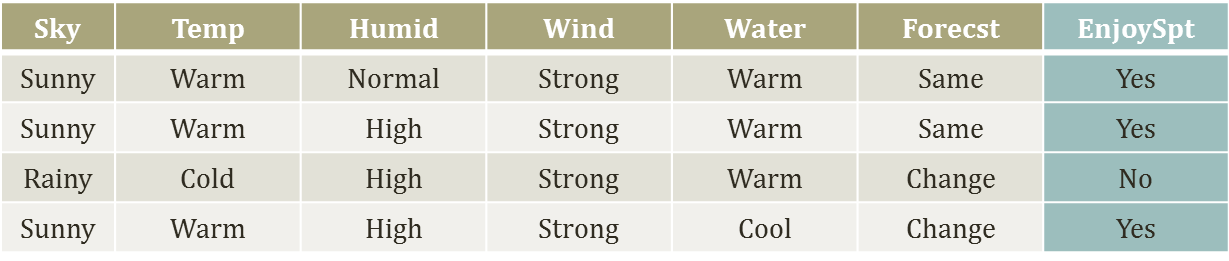
\includegraphics[scale=0.5]{Dataset}\caption{데이터셋}\label{Fig:3-9}
\end{figure}
이제 앞서 나왓던 데이터셋을 다시 다뤄보겠다. 앞서 다뤘던 최적 분류기(Optimal Classifier) $f^*(x)$는 다음과 같았다.
$$f^*(x) = {argmax}_Y=y P(X = x|Y = y)P(Y = y)$$
그리고 여기서 $P(X=x|Y=y)$에 필요한 매개변수의 수는 $(2^d -1)k$개의 경우로 매우 많았다. 그래서 여기서 X의 모든 요소들(x벡터의 모든 변수)에 조건부 확률을 가정해 접목시켜보겠다. 이 경우 $P(X = x|Y = y)$부분이 바뀌어 다음과 같은 식으로 유도할 수 있다.
\begin{equation}
\begin{split}
f^*(x) &= {argmax}_{Y=y} P(X = x|Y = y)P(Y = y) \\
&\approx {argmax}_{Y=y}P(Y=y) \prod_{1\le i \le d} P(X_i = x_i|Y=y)
\end{split}
\label{eq:1-22}
\end{equation}
이와 같이 조건부 확률을 가정하고 나서는 $P(X_i = x_i|Y = y)$에 필요한 매개변수의 수가 확 줄어들게 된다. 앞서 각 요소들은 2개의 경우만 있다고 가정을 했으므로 1개의 경우만 있으면 나머지 한개의 경우를 유추할 수 있고 $x_i$는 d개가 있고, $Y$는 k개의 경우가 있으므로 $(2-1)dk$개의 경우만 있으면 된다. 그렇지만 수식 \eqref{eq:1-22}가 정확한 등호는 아니다. 이 이유는 조건부 독립을 가정했기 때문이다.

% 슬라이드 17
이와 같은 가정은 매우 순진한(Naive) 가정이다. 그래서 이런 분류기를 나이브 베이즈 분류기(Naive Bayes Classifier)라고 부르게 되었다. 그래서 $P(Y)$라는 사전 클래스가 주어졌고, $Y$ 클래스 조건에서 $X$에는 $d$개의 조건부 독립인 특성 $X_i$이 주어졌다고 생각을 해보자. 그리고 각각의 $X_i$에 대해서 $P(X_i|Y)$의 우도(Likelihood)를 가지고 있다고 생각을 해보자. 이때 나이브 베이즈 분류기 함수는 다음과 같다.
\begin{equation}
f_{NB}(x)={argmax}_{Y=y}P(Y=y)\prod_{1\leq i \leq d}P(X_i=x_i|Y=y)
\label{eq:1-23}
\end{equation}
\indent 나이브 베이즈 분류기(Naive Bayes Classifier)는 X가 조건부 독립 가정을 만족하고, 사전 정보도 맞다면 최적 분류기(Optimal Classifier)이다. 그렇다면 나이브 베이즈 분류기의 문제점은 무엇일까?\\\\

% 슬라이드 18
\subsection{나이브 가정(Naive assumption)}
나이브 베이즈 분류기는 MLE, MAP를 이용하면 만들기가 쉽다. 하지만 쉬운 만큼 문제점도 있다. 첫번째 문제점은 순진한(Naive) 가정이라는 것이다. 현실에서는 대부분의 경우 X의 특성들이 서로 상관관계를 가지는 경우가 많다. 그래서 다중공선성(multi-collinearity)를 가지는 경우도 있다. 두번째 문제점은 부정확한 확률 추정이라는 것이다. 압정 문제에서 백만장자가 준 데이터가 모두 다 앞면이 나왔다고 한다면 이는 불충분한 데이터의 MLE로써, 뒷면이 나올 기회가 없게 된다. 즉 $P(Y=tail)=0$가 된다. MAP의 경우에 엉터리 사전 정보가 주어질 경우 문제가 생긴다. 우리가 가지고 있는 데이터셋이나 지식이 사전 정보를 추정하기에 충분한지에 대한 의문을 가져야 한다.\\
\indent 두번째 문제점의 경우에는 항상 존재하는 문제점이다. 하지만 첫번째 문제점은 우리가 나이브 베이즈 분류기의 형태를 만들기 위해 도입한 가정으로 정확할 필요가 있다. 후에 로지스틱 회귀분석(Logistic regression)에 대해서 다룰 때 나이브(Naive) 가정을 없애는 방향으로 해볼 예정이다. \\
\indent 이렇게 나이브 베이즈 분류기에 대해서 알아봤는데 나이브 베이즈 분류기는 나이브 가정을 쓴다는 문제점을 가지고 있다. 이는 Bayes Theorem을 쓰는 순간부터 예고가 되었던 부분이었는데, 뒤에서 로지스틱 회귀분석(Logistic regression)을 활용하여 나이브 가정을 도입하지 않고 분류기를 만드는 방법을 알아보도록 하겠다. 그 전에 나이브 베이즈 분류기를 텍스트마이닝에 접목하는 방법에 대해서 알아보도록 하겠다.\\\\
 
% 슬라이드 20
\section{사례 연구}
이번에는 나이브 베이즈 분류기를 텍스트마이닝에 적용해보도록 하겠다. 텍스트마이닝은 많은 분야에서 적용을 하고 있다. 예를 들어 하나를 살펴보면, 아마존이라는 물건을 파는 사이트에 가보면 사람들이 상품에 대한 평가를 남겨놓는다. \\
\begin{figure}[ht]\centering
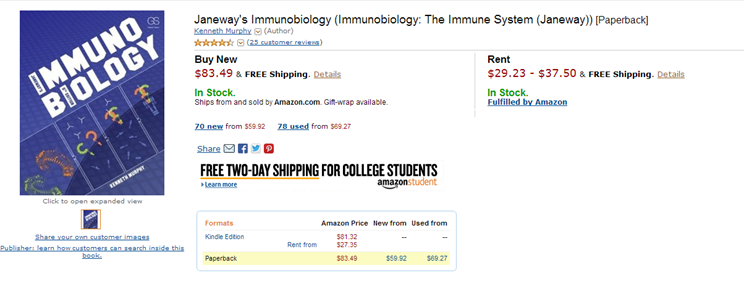
\includegraphics[scale=0.8]{Amazon}\caption{아마존의 상품}\label{Fig:3-10}
\end{figure}
\begin{figure}[ht]\centering
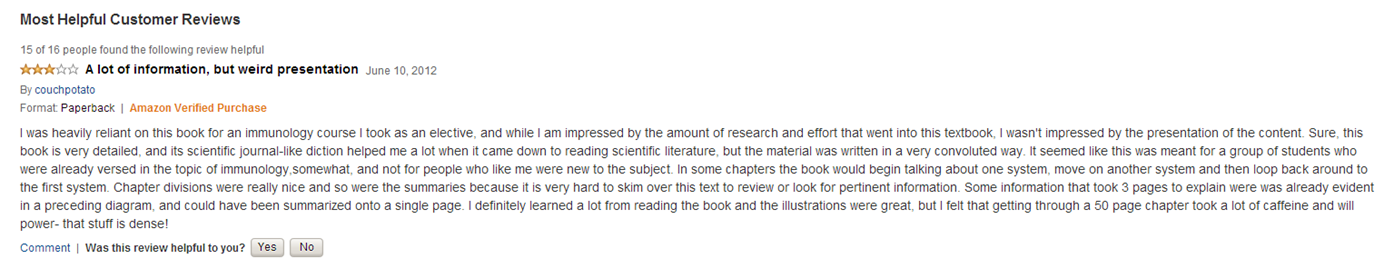
\includegraphics[scale=0.5]{Amazon_review}\caption{상품에 대한 리뷰}\label{Fig:3-11}
\end{figure}\\
\indent 예를 들어 그림 10과 같이 책을 팔고 있을 때 그림 11과 같이 리뷰가 달려있다. 리뷰들 중에는 긍정적인 리뷰도 있을 수 있고 부정적인 리뷰도 있을 수 있다. 상품 개발자는 자신의 상품을 개선시키기 위해 소비자들의 피드백을 받고 싶을 것이다. 하지만 만약 리뷰가 10,000개 있다면 상품 발전을 위해 부정적인 리뷰를 일일히 찾아보는 것은 비효율적일 것이다. 이 때 인공지능을 활용하여 부정적인 리뷰를 찾아주는 프로그램을 만드면 좋을 것이다. 그렇다면 어떻게 이런 모델을 만들 수 있을까?\\

% 슬라이드 21
\indent 바로 나이브 베이즈 분류기를 적용할 수 있을 것이다. 그렇지만 `훌륭하다',`좋다',`완벽하다'나 `끔찍하다',`최악이다',`절대 안산다'와 같이 구분히 확실히 되는 단어로만 찾는 것은 다양한 상품평을 정확히 분류하는 것은 어려울 것이다. 예를 들어, 레스토랑의 리뷰에서 피자가 `차갑다'는 말에서는 `차갑다'가 부정적인 의미로 쓰인 것이다. 하지만 맥주의 리뷰에서는 `차갑다'란 말이 긍정적인 의미로 쓰일 수 있다. 즉, 긍정적인지 부정적인지 확연히 알아볼 수 있는 단어가 아닌 `차갑다', `뜨겁다'와 같이 특성을 나타내는 단어를 부정적인 리뷰를 찾는 데 쓰기 위해서는 좀 더 전문적인 분류기(Classifier)가 필요할 것이다.
\begin{figure}[ht]\centering
\parbox[t]{4cm}{
\includegraphics[scale=0.5]{Pizza}\caption{차가운 피자}\label{Fig:3-12}}\hspace{1cm}
\parbox[t]{4cm}{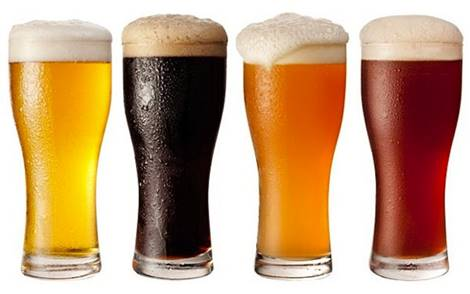
\includegraphics[scale=0.5]{Beer}\caption{차가운 맥주}\label{Fig:3-13}}
\end{figure}
\begin{figure}[ht]\centering
\parbox[t]{4cm}{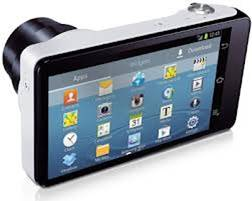
\includegraphics[scale=0.5]{LCD}\caption{카메라 LCD}\label{Fig:3-14}}\hspace{1cm}
\parbox[t]{4cm}{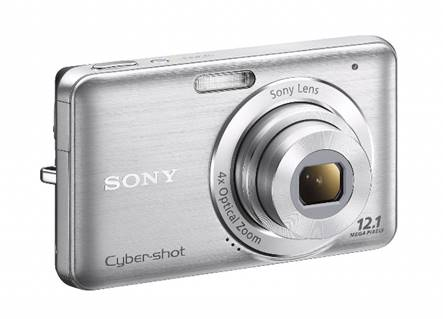
\includegraphics[scale=0.5]{Camera}\caption{카메라 크기}\label{Fig:3-15}}
\end{figure}\\
\indent 또 다른 예시로 카메라의 크기는 작을수록 좋지만, LCD화면은 클수록 좋을 것이다. 그래서 `크다', `작다'와 같은 단어들도 상품에 대한 질을 표현하고 있지만 어떻게 쓰이느냐에 따라 리뷰의 의미가 달라질 수 있다. 이러한 것을 감안한 기계학습 모델을 만들어 보고자 한다. 물론 나이브 베이즈 분류기만으로 이러한 것이 잘 되는 모델을 만들기는 힘들다. 그래도 실제 데이터셋에 나이브 베이즈 분류기를 적용을 시켜보고자 한다.

% 슬라이드 22
\subsection{Bag of Words}
먼저 통계적인 분석을 위해서는 텍스트 형태인 리뷰를 벡터 형태로 변환을 하는 것이 좋다. 기계학습이라고 하는 것은 $D$라는 데이터에서 매개변수 $\theta$를 찾아내는 과정이다. 그 말은 즉슨, $\theta$를 찾기 위해서는 $D$라는 데이터가 필요하다. 그래서 $D$라는 데이터가 컴퓨터 속에서 어떻게 표현되는 지를 알아야 한다. 앞서 그림 9에서 데이터셋은 각 요소별로 값들이 정해져 있었다. 하지만 텍스트 형태의 리뷰는 그렇지 않다. 그렇다면 텍스트 형태의 리뷰는 어떻게 데이터셋으로 만들 수 있을까?\\
\indent 바로 Bag of words 기법을 이용하면 된다. 먼저 단어 리스트를 벡터 형태로 만든다. 예를 들어 $<I, cool, led, reliant>$와 같이 4개의 단어가 들어 있는 리스트를 만들어 보자. 그리고 각 리뷰에 대해서 이 단어들이 포함되어 있는지 판단해 단어가 포함되어 있다면 1의 값을 주고 포함되어 있지 않다면 0의 값을 주어 새로운 벡터를 만들 수 있다. 그림 16의 리뷰의 경우에는 $<I, cool, led, reliant>$ 단어 리스트에 대한 벡터는 $<1,0,0,1>$이 될 것이다.
\begin{figure}[ht]\centering
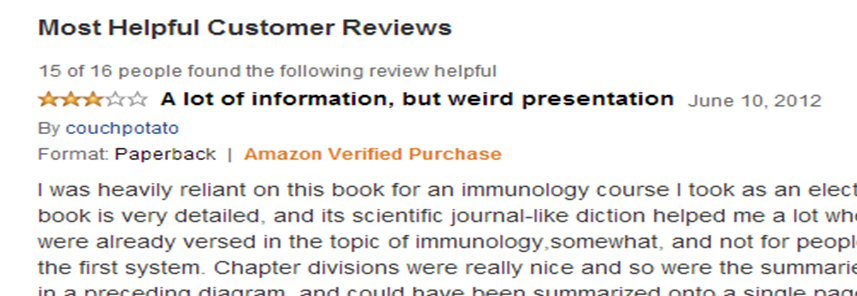
\includegraphics[scale=0.5]{Review_Example}\caption{리뷰 예시}\label{Fig:3-16}
\end{figure}\\
\indent 한편 단어의 포함 여부가 아닌 단어의 등장 횟수로 벡터를 나타낼 수도 있다. 이런식으로 하나의 텍스트 형태의 리뷰를 수치적인 정보로  변환하는 과정을 거치는데 이를 Bag of words라고 부른다.\\\\

% 슬라이드 23
\subsection{Classifier를 통한 문서 분류 방법}
\indent 필자는 이런 방법으로 한 상품에 대하여 198개의 리뷰에 대해서 Bag of words를 구해보았다. 그 결과 29,717 개의 고유의 단어가 존재하였다. 그리고 클래스는 긍정적인 감정과 부정적인 감정으로 나눠 보았다. 이제 이 데이터셋을 나이브 베이즈 분류기에 적용을 해보겠다. 나이브 베이즈 분류기의 식은 다음과 같았다.
$$f_{NB}(x)={argmax}_{Y=y}P(Y=y)\prod_{1\leq i \leq d}P(X_i=x_i|Y=y)$$
여기서 Y의 클래스는 긍정적인 감정과 부정적인 감정으로 2개의 클래스가 존재한다. 그리고 리뷰 X의 요소는 단어리스트의 각 단어들의 등장여부에 따라 0이나 1의 값이 주어진다. 물론 여기서 `LCD'와 `카메라'와 같이 서로 연관관계가 깊은 단어들이 있을 수 있다. 하지만 나이브 베이즈 분류기는 순진한(Naive) 가정으로 각 단어들이 조건부 독립이라는 가정을 넣으므로 이런 상황을 무시하게 된다.\\
\indent 즉, 우리는 2 종류의 확률을 구해야한다. 한 종류는 사전정보로 $P(Y=y)$값이고 다른 한 종류는 우도(Likelihood)로 $P(X_i=x_i|Y=y)$값이 된다. 이것을 MLE나 MAP로 계산을 하면 전체 $P(Y=y)\prod_{1\leq i \leq d}P(X_i=x_i|Y=y)$ 값을 계산을 할 수 있고, 이 값은 긍정적인 감정에 대한 계산을 할 수도 있고 부정적인 감정에 대해서 계산을 할 수도 있다. 각 리뷰에 대해서는 두 값을 구한 뒤 좀 더 높은 값을 가지는 쪽이 긍정적인쪽인지 부정적인쪽인지 비교하여 분류를 할 수 있을 것이다.\\

% 슬라이드 24
\subsection{Matlab exercise}
\indent 이 방법을 이용하여 matlab으로 프로그램을 구현해 보았다. \\
\indent 이런 나이브 베이즈 분류기는 기계학습 알고리즘 중 가장 쉬운 알고리즘이다. 다음 장에서는 순진한 가정을 넣지 않고 $P(Y|X)$를 그대로 유지해서 분류를 해보는 로지스틱 회귀분석(Logistic regression) 모델을 배워보도록 하겠다. 

% 슬라이드 25
\section*{Acknowledgement}
\noindent This slideset is greatly influenced by
\begin{itemize}\setlength\itemsep{-\parsep}
\item Professor Eric P. Xing at CMU
\end{itemize}

% 슬라이드 26
\section*{Further Readings}
\begin{itemize}
\setlength\itemsep{-\parsep}
\item Bishop Chapter 1, 8.2
\end{itemize}
\end{document}
